% The Visual Computer (Springer) -- single-column manuscript.
% Build: pdflatex main && bibtex main && pdflatex main && pdflatex main
\documentclass[11pt,a4paper]{article}
\usepackage[margin=2.6cm]{geometry}
\usepackage{amsmath,amssymb,amsthm,bm,booktabs,graphicx,url,makecell}
\usepackage[hidelinks]{hyperref}
\usepackage[nameinlink,noabbrev]{cleveref}
\graphicspath{{../figures/}}
\setlength{\emergencystretch}{1em}
\newtheorem{proposition}{Proposition}
\newcommand{\R}{\mathbb{R}}
\newcommand{\Sstate}{\mathbf{S}}
\newcommand{\vect}{\operatorname{vec}}

\title{\bfseries A fixed-state additive FWP network for streaming point-cloud
recognition}
\author{Dian Yu\thanks{Corresponding author. \texttt{dian.yu2@student.unsw.edu.au},
ORCID \url{https://orcid.org/0009-0002-0107-1014}}\\[2pt]
\normalsize University of New South Wales, Sydney, NSW 2052, Australia}
\date{}

\begin{document}
\maketitle

\begin{abstract}
\noindent
Most point-cloud networks obtain context by revisiting stored points, rebuilding neighborhoods, or applying a global maximum. These operations are effective offline but make a growing stream dependent on its history. PointProgrammerNet replaces point history with three fixed $128\times170$ matrices. For every observation, a normalized spatial address specifies where to write and a value vector specifies what to write; their outer product is added to each matrix. This simple construction makes independently encoded chunks exactly mergeable by matrix addition and also permits subtraction and exponential decay. Segmentation reads the matrices at a requested coordinate, while classification uses the matrices alone after all points have been discarded. We prove order invariance, chunk and distributed equivalence, fixed retained memory, and continuous dependence on incoming evidence. With XYZ input, the model obtains $92.95\%$ point accuracy, $82.58\%$ instance mIoU, and $79.10\%$ category mIoU on ShapeNetPart, and $86.59\%$ accuracy on ModelNet40. The three float32 states occupy 255 KiB regardless of stream length. At 8,192 accumulated points, updating one new chunk is $6.06\times$ faster than rebuilding the complete state, while the relative state error remains below $10^{-6}$. The results show the accuracy cost and operational benefit of replacing an expanding point history with a bounded state that can be updated and combined directly.
\end{abstract}

\noindent\textbf{Keywords:} point clouds; streaming learning; additive state;
fast-weight programmers; segmentation; classification

\section{Introduction}
A point cloud is an unordered set, but a sensor observes it over time. Processing within a frame should be independent of point order, and processing across frames should not require replaying the full history. PointNet~\cite{qi2017pointnet} obtains a global descriptor by symmetric maximum pooling, while PointNet++~\cite{qi2017pointnetplusplus} builds multiscale metric neighborhoods. Both are effective offline. However, a maximum is not an additive state: fixed summaries cannot generally support deletion, independent chunk merging, and continuously weighted evidence by simple addition.

We study a stricter setting in which a point may be discarded immediately after it is written. Later computation accesses only fixed matrices, plus a query coordinate for segmentation. A learned key distributes each point across state rows, and a second-order value records mass, position, learned content, and cross moments. Summing these per-point writes produces a fixed-size state.

Independent chunks can therefore be merged, a stored subset can be subtracted, and old evidence can be decayed. New points update the state without a pass over earlier observations. The same algebra supports distributed sensing: edge devices encode disjoint regions or time windows, transmit fixed matrices, and a central node adds those matrices before classification or segmentation. Segmentation reads a coordinate-conditioned field and stores no historical point features. Classification reads only state rows and discards the complete point list.

Our contributions are:
\begin{itemize}
\item a three-scale second-order fast-weight-programmer (FWP) state whose memory does not grow with the number of observed points;
\item additive point writes that support exact streaming, hierarchical merging, and distributed aggregation without replaying chunk contents, and that admit a fully parallel write and read;
\item a coordinate-conditioned segmentation head and a state-only classification head, neither of which pools over decoded points;
\item proofs and experiments covering additivity, state operations, accuracy, and update cost, including a causal test showing that three parallel states outperform one state at an equal parameter budget.
\end{itemize}

\section{Related Work}
There are several established ways to reduce an unordered point set to a fixed summary. They differ mainly in what they give up at the moment a point is absorbed, and that choice decides which state operations remain available afterwards. We group the related work by that choice, then state which properties this architecture keeps.

\subsection{Symmetric pooling and metric neighborhoods}
PointNet applies pointwise transforms followed by maximum pooling~\cite{qi2017pointnet}, PointNet++ adds hierarchical metric neighborhoods~\cite{qi2017pointnetplusplus}, and Deep Sets characterizes permutation-invariant functions built from sums~\cite{zaheer2017deepsets}. All three are invariant to point order, and the sum used by Deep Sets is additive in the strict sense of Equation~\eqref{eq:add-main}. A growing stream nevertheless runs into two obstacles. A channelwise maximum discards the information needed to undo it, so a stored summary cannot be corrected once an observation is removed. A metric neighborhood is defined relative to the points currently held; insert or delete one point and the membership of other neighborhoods shifts with it, forcing the grouping to be rebuilt. Deep Sets escapes both, at the price of summing into a single global vector that carries no spatial address and cannot be evaluated at a requested coordinate. We keep the additive sum but spread it over 128 spatially addressed rows, so a coordinate-conditioned read remains possible without giving up additivity.

\subsection{Fixed-size summaries over learned centers}
VLAD compresses local descriptors by assigning them to learned centers and accumulating residuals~\cite{jegou2010vlad}. NetVLAD makes that assignment soft and differentiable~\cite{arandjelovic2016netvlad}, and PointNetVLAD applies the construction to point clouds for place recognition~\cite{uy2018pointnetvlad}. The accumulator has the same shape as ours: a fixed matrix built by soft assignment to learned centers. It differs in what is accumulated and in what happens afterwards. The residuals are first order, whereas Equation~\eqref{eq:value-main} retains every moment up to second order, and the assignment is made in feature space, whereas our address is a normalized function of the coordinate and stays continuous in a query position. The decisive difference is the last step. NetVLAD intra-normalizes each block and then $L_2$-normalizes the flattened descriptor, and neither operation is additive: normalizing two partial descriptors and adding them does not reproduce the descriptor of their union. The raw accumulator is additive, but the published construction normalizes that property away and never uses it. We leave the accumulator unnormalized and move normalization to read time, preserving \Cref{prop:order}.

\subsection{Attention over a fixed latent set}
Set Transformer summarizes a set using inducing points and attention~\cite{lee2019settransformer}. Perceiver IO maintains a latent array whose size is independent of the input and decodes arbitrary outputs, including dense per-element predictions, by attending to that latent with an output query array~\cite{jaegle2022perceiverio}. Reading a fixed latent with a query in order to produce dense output is their contribution, not ours. The difference lies on the encoding side. Softmax cross-attention normalizes over the observed elements, so the latent obtained from two disjoint chunks is not the sum of the two latents; the representation cannot be merged, subtracted, or decayed arithmetically, and no such property is claimed. Our write applies no normalizer over the observed set, so the state remains a sum of independent per-point terms. The meaning of a query also differs: Perceiver queries are learned position embeddings, whereas ours is a coordinate in the same space as the data, so one state can be evaluated at positions that were never observed.

\subsection{Bounded recurrent state}
Kernelized attention can be evaluated recurrently with a fixed-size state~\cite{katharopoulos2020transformers}, and fast-weight programmers express such updates as additive outer products or delta corrections~\cite{schlag2021linear}. These are the mechanisms our write uses. Recent point-cloud work also adopts a bounded state through structured state space models; PointMamba serializes points with space-filling curves before the recurrence~\cite{liang2024pointmamba}. Serialization makes the hidden state a function of the traversal order, so it is not permutation invariant and two partial states cannot be added. We keep the bounded state but not the sequence: chunk and device equivalence rests on the sum being order free.

\subsection{What this architecture refuses to do}
Every family above trades one property for another: a maximum gives up invertibility, a metric neighborhood gives up locality of edits, a normalized descriptor gives up additivity, a softmax encoder gives up decomposability, and a serialized recurrence gives up order invariance. The design studied here follows from a single refusal at write time: nothing that couples one point's write to another point may enter the persistent state. That excludes normalization over the observed set, comparison between points, selection, and ordering. Operations that aggregation methods usually perform while absorbing a point --- density normalization, centring on a reference position, and nonlinear interpretation --- are instead deferred to the read, where they no longer touch the algebra of the stored matrices. \Cref{tab:family-comparison} states the resulting position.

\begin{table}[t]
\centering
\caption{Properties retained by families of set summaries. ``Order-free write'' means the summary does not depend on the order in which points are absorbed; ``additive state'' means the summary of a union equals the sum of the summaries; ``bounded state'' means retained memory does not grow with the number of observed points; ``coordinate read'' means the summary alone can be evaluated at a requested position.}
\label{tab:family-comparison}
\small
\begin{tabular}{lcccc}
\toprule
Family & \makecell{Order-free\\write} & \makecell{Additive\\state} & \makecell{Bounded\\state} & \makecell{Coordinate\\read} \\
\midrule
PointNet, maximum pooling & yes & no & yes & no \\
PointNet++, metric neighborhoods & yes & no & no & no \\
Deep Sets, global sum & yes & yes & yes & no \\
VLAD, NetVLAD, PointNetVLAD & yes & no$^{a}$ & yes & no \\
Set Transformer, inducing points & yes & no$^{b}$ & yes & no \\
Perceiver IO, output queries & yes & no$^{b}$ & yes & yes$^{c}$ \\
Linear attention, fast weights & yes$^{d}$ & yes & yes & no \\
State space models on serialized points & no & no & yes & no \\
\midrule
PointProgrammerNet (this work) & yes & yes & yes & yes \\
\bottomrule
\end{tabular}
\\[3pt]
\parbox{\linewidth}{\footnotesize $^{a}$The raw accumulator is additive, but intra-normalization and $L_2$ normalization remove the property. $^{b}$Softmax over the observed elements couples them. $^{c}$Perceiver IO decodes dense outputs from learned position queries, not from a coordinate in the input space. $^{d}$The outer-product update is itself order free, although these models are applied to ordered sequences.}
\end{table}

What that refusal provides and what it costs are both measured rather than asserted. \Cref{sec:parallel} isolates the contribution of the parallel-state structure, and \Cref{tab:segmentation_accuracy,tab:classification_accuracy} place the resulting accuracy against hierarchical baselines.

We evaluate classification on ModelNet40~\cite{wu20153dshapenets} and part segmentation on ShapeNetPart~\cite{yi2016scalable}, which is derived from ShapeNet~\cite{chang2015shapenet}.

\section{Method}
Let $X=\{\bm{x}_i\}_{i=1}^N$, with normalized coordinates $\bm{x}_i\in\R^3$. PointProgrammerNet replaces the growing point history with three matrices $\Sstate_s\in\R^{128\times170}$, where $s\in\{f,m,b\}$ denotes branches initialized at radii $0.08$, $0.20$, and $0.60$. The radii, spatial centers, point encoders, and read networks are learned independently. The state is created for each object or stream and is separate from the trained model parameters.

All three branches have the same state dimensions and use the same equations. Their different initial radii only provide distinct starting conditions; the trained network decides what each branch represents. A branch first maps a coordinate to learned content with a two-layer point network,
\begin{equation}
\bm g_s(\bm x)=\operatorname{ReLU}\!\left(\operatorname{BN}\!\left(W_{s2}
\operatorname{ReLU}(\operatorname{BN}(W_{s1}\bm x+\bm b_{s1}))+\bm b_{s2}\right)\right)
\in\R^{32}.
\label{eq:content-main}
\end{equation}
The matrices $W_{s1},W_{s2}$ and biases are learned separately in each branch, and both hidden layers have width 32. Consequently, equal state sizes do not imply repeated features.
This nonlinear map is evaluated independently for each point. It therefore enriches what a point writes without coupling that write to any other point; additivity is preserved because only the subsequent outer products are accumulated in the persistent state.

\begin{figure}[t]
\centering
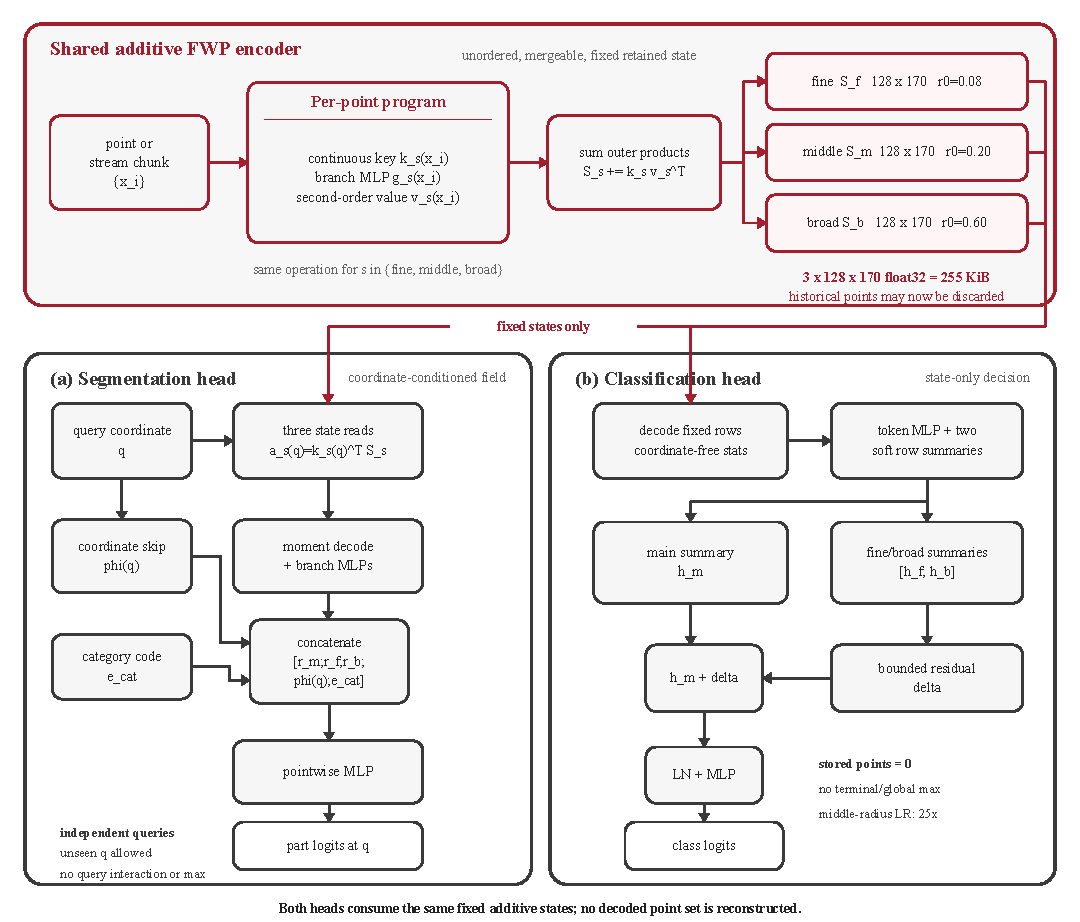
\includegraphics[width=\linewidth]{fig00_pointprogrammernet_architecture.pdf}
\caption{PointProgrammerNet architecture. Red paths carry the three equal-size additive FWP states after historical points have been discarded. The segmentation head reads each state at query coordinate $\bm q$, then concatenates the decoded context, coordinate skip, and category code. The classification head decodes fixed rows and adds a bounded fine--broad residual to the middle-state summary. Neither head reconstructs or pools over a decoded point set.}
\label{fig:architecture}

\end{figure}

\subsection{Additive state construction}
Each of the 128 state rows has a learned center $\bm c_{sj}\in\R^3$. These centers are not sampled from an input cloud. Before training, a Sobol sequence simply places 128 initial anchors across $[-0.9,0.9]^3$ so that the rows begin with broad spatial coverage. Every branch receives its own trainable copy, and training may move the anchors through the bounded parameterization $\bm c_{sj}=0.95\tanh(\bm\theta_{sj})$. For one observed coordinate $\bm x$, the branch measures its distance to all 128 anchors and converts those distances into 128 continuous write fractions. The positive radius $r_s=\exp(-\lambda_s)$ controls how concentrated these fractions are. The normalized address is
\begin{equation}
k_{sj}(\bm x)=\frac{\exp[-\|\bm x-\bm c_{sj}\|^2/(2r_s^2)]}
{\sum_{u=1}^{128}\exp[-\|\bm x-\bm c_{su}\|^2/(2r_s^2)]}.
\label{eq:key-main}
\end{equation}
The denominator fixes every point's total write mass at one. This prevents dense chunks from changing the scale of an individual write and lets the radius control concentration rather than total magnitude. In practical terms, the centers act like 128 soft spatial bins. A point near several centers gives those rows large fractions and all other rows small fractions; it is never assigned to only one bin. The address determines where the point contributes, while the following 170-dimensional value determines what statistics it contributes:
\begin{equation}
\bm v_s(\bm x)=[1,\bm x,\bm g_s,\vect(\bm x\bm g_s^\top),
 x^2,y^2,z^2,xy,xz,yz,\bm g_s\odot\bm g_s].
\label{eq:value-main}
\end{equation}
The blocks have dimensions $1+3+32+96+6+32=170$ and retain mass, first moments, learned content, coordinate--content products, and second moments. The leading one later supplies the denominator for local averages. The six quadratic coordinate terms and 32 squared feature terms retain spread that cannot be recovered from a mean. Equivalently, the value vector collects every moment of $(\bm x,\bm g_s)$ up to second order, with the feature--feature block restricted to its diagonal so that its width stays linear in the content dimension.
\begin{table}[t]
\centering
\caption{The value written by one point. Every state row has these 170 columns.}
\label{tab:value-layout-main}
\begin{tabular}{lrl}
\toprule
Block & Dim. & Information retained \\
\midrule
$1$ & 1 & accumulated mass \\
$\bm x$ & 3 & coordinate sum \\
$\bm g_s$ & 32 & learned-content sum \\
$\bm x\bm g_s^\top$ & 96 & position--content relation \\
$\bm x\bm x^\top$ & 6 & geometric second moment \\
$\bm g_s\odot\bm g_s$ & 32 & feature second moment \\
\bottomrule
\end{tabular}
\end{table}
A point changes state row $j$ by
\begin{equation}
[\Delta\Sstate_s(\bm x)]_{j,:}=k_{sj}(\bm x)\bm v_s(\bm x)^\top .
\label{eq:single-write-main}
\end{equation}
This rank-one update uses the defining FWP operation: the key selects where to write, the value supplies what to write, and independent writes superpose by addition~\cite{schlag2021linear}. PointProgrammerNet preserves this linear superposition, without a write normalization over the observed point set or a nonlinear overwrite of the previous state. Thus a row is a weighted accumulator rather than a slot for one selected point, and summing the outer products gives
\begin{equation}
\Sstate_s(X)=\sum_{i=1}^{N}\bm k_s(\bm x_i)\bm v_s(\bm x_i)^\top
=\bm K_s^\top\bm V_s.
\label{eq:state-main}
\end{equation}
No point is assigned to a single row and no point is compared with another point. Once its three outer products have been added, it may be released.

For a newly arrived chunk, $\bm K_s\in\R^{M\times128}$ stacks its addresses and $\bm V_s\in\R^{M\times170}$ stacks its values. The chunk update is one matrix product $\Delta\Sstate_s=\bm K_s^\top\bm V_s$. The persistent state is updated by $\Sstate_s\leftarrow\Sstate_s+\Delta\Sstate_s$, after which $\bm K_s$, $\bm V_s$, and the chunk points can be discarded. Chunk size changes temporary working memory, but not the retained representation.

The complete streaming workflow is therefore short. For each arriving chunk, the encoder (i) normalizes its coordinates in the shared reference frame, (ii) computes the three address and value matrices, (iii) adds the three products $\bm K_s^\top\bm V_s$ to the persistent states, and (iv) releases all chunk-dependent tensors. Independent devices perform the same four steps and transmit only their three matrices. At inference, the segmentation head evaluates only requested coordinates, whereas the classification head consumes the matrices directly. No later stage needs to regenerate a point list from the state.

\subsection{Task readouts}
For segmentation, $\bm x_i$ denotes an observed point that has already been added to the state and may then be discarded; $\bm q$ is only the coordinate at which a label is requested. On ShapeNetPart, queries use the labeled input coordinates, but the decoder receives the coordinate and fixed state rather than the stored point feature. A query produces an address by Equation~\eqref{eq:key-main} and reads
\begin{equation}
\bm a_s(\bm q)=\bm k_s(\bm q)^\top\Sstate_s
=\sum_i \underbrace{\bm k_s(\bm q)^\top\bm k_s(\bm x_i)}_{w_{si}(\bm q)}
\bm v_s(\bm x_i)^\top .
\label{eq:effective-read-main}
\end{equation}
The coefficient $w_{si}(\bm q)$ is an algebraic interpretation of the matrix read: it is large when point $i$ wrote strongly to rows that $\bm q$ reads strongly. The implementation evaluates the left-hand matrix product directly; it neither reconstructs or revisits point $i$ nor applies a global maximum over decoded points.

The first component of $\bm a_s(\bm q)$ is the read mass $\mu_s(\bm q)$. The implementation prevents unstable division in nearly empty regions with
\begin{equation}
\epsilon_s=10^{-3}\operatorname{mean}_{\bm q'}\mu_s(\bm q')+10^{-20},
\qquad
\widetilde\mu_s(\bm q)=\max(\mu_s(\bm q),\epsilon_s).
\label{eq:seg-floor}
\end{equation}
The mean is taken over the query coordinates of one sample and is detached from the gradient. The maximum in Equation~\eqref{eq:seg-floor} is only a scalar numerical floor; it neither compares point features nor performs global maximum pooling. Dividing the stored coordinate, feature, cross-product, and square sums by $\widetilde\mu_s$ yields local coordinate and feature means $\bar{\bm x}_s,\bar{\bm g}_s$, cross moment $E_{xg,s}$, geometric moment $E_{xx,s}$, and feature energy $E_{gg,s}$. They form the 170-dimensional descriptor
\begin{equation}
\begin{aligned}
\bm d_s(\bm q)=[&\bar{\bm g}_s,\bar{\bm x}_s-\bm q,\log\widetilde\mu_s,
\vect(E_{xg,s}-\bm q\bar{\bm g}_s^\top),\\
&\operatorname{vech}(E_{xx,s}-\bar{\bm x}_s\bar{\bm x}_s^\top),
\sqrt{[E_{gg,s}-\bar{\bm g}_s\odot\bar{\bm g}_s]_++10^{-8}}].
\end{aligned}
\label{eq:query-descriptor-main}
\end{equation}
Here $\operatorname{vech}$ keeps the six distinct entries of a symmetric $3\times3$ matrix, and $[\cdot]_+$ clips roundoff-induced negative variances. Its block dimensions are $32,3,1,96,6,32$, again totalling 170. The descriptor deliberately combines complementary statistics. The feature mean supplies local semantic content, the relative centroid and geometric covariance describe local position and shape, and the log mass records how much evidence supports the read. The coordinate--feature term preserves how content changes around the query, while the feature standard deviation exposes mixtures and boundary variation that a mean alone would hide. Each branch applies the same $170\rightarrow160\rightarrow160$ BatchNorm--ReLU decoder. The final pointwise head is
\begin{equation}
\bm z_{\rm seg}(\bm q)=h_{\rm seg}([\bm r_f(\bm q);\bm r_m(\bm q);
\bm r_b(\bm q);\phi(\bm q);\bm e_{\rm cat}]),
\label{eq:seg-main}
\end{equation}
where $\bm r_s\in\R^{160}$ is a decoded state read, $\phi(\bm q)\in\R^{32}$ is a coordinate feature, and $\bm e_{\rm cat}\in\R^{16}$ is the ShapeNetPart category code. The segmentation MLP is $528\rightarrow256\rightarrow128\rightarrow50$, with BatchNorm, ReLU, and dropout $0.3$ after its first two affine layers. The coordinate path is a U-Net-like skip around state compression. The head acts on each query separately and never pools over decoded points. Historical features can be deleted; only coordinates that will later be labelled must remain. The same fixed state can also be queried at an unobserved coordinate.

For classification, no coordinates are retained. For row $j$, the 170 stored entries are partitioned as
\[
[\mu_{sj},\bm p_{sj},\bm f_{sj},\vect(\bm C_{sj}),
\operatorname{vech}(\bm Q_{sj}),\bm u_{sj}],
\]
that is, mass, coordinate sum, feature sum, coordinate--feature sum, symmetric coordinate second moment, and squared-feature sum. Row normalization uses
\begin{equation}
\widetilde\mu_{sj}=\max\!\left(
\mu_{sj},10^{-4}R^{-1}\sum_{u=1}^{R}|\mu_{su}|+10^{-20}\right),
\label{eq:cls-floor}
\end{equation}
whose lower bound is detached during back-propagation. With $\bar\mu_s=R^{-1}\sum_u\widetilde\mu_{su}$, division by $\widetilde\mu_{sj}$ produces
\begin{equation}
\begin{aligned}
\bm d^{\rm row}_{sj}=[&
\bar{\bm g}_{sj},\bar{\bm x}_{sj},
\log(\widetilde\mu_{sj}/\bar\mu_s),
\operatorname{vech}(\operatorname{Cov}_{xx,sj}),\\
&\operatorname{Std}_{g,sj},
\vect(\operatorname{Cov}_{xg,sj})]\in\R^{170},
\end{aligned}
\label{eq:cls-descriptor}
\end{equation}
with block dimensions $32,3,1,6,32,96$. An independent $170\rightarrow128\rightarrow128$ LayerNorm--GELU network encodes every row, giving $\bm T_s\in\R^{128\times128}$. Two learned score columns summarize the fixed rows:
\begin{equation}
\bm U_s=\operatorname{softmax}_{\rm rows}(\operatorname{score}_s(\bm T_s)),\qquad
\bm h_s=H_s(\vect(\bm U_s^\top\bm T_s))\in\R^{256}.
\label{eq:state-summary-main}
\end{equation}
This softmax is over 128 retained state rows, not over the input points, so its cost is fixed after encoding. The middle summary is the reference and the other two form a bounded residual:
\begin{align}
\bm\delta&=\sigma(a)\tanh(W[\bm h_f;\bm h_b]+\bm b),\nonumber\\
\bm z_{\rm cls}&=h_{\rm cls}(\operatorname{LN}(\bm h_m+\bm\delta)).
\label{eq:cls-main}
\end{align}
The residual projection starts at zero and $\sigma(a)$ starts at $0.1$. The classifier $h_{\rm cls}$ is $256\rightarrow256\rightarrow40$, with GELU and dropout $0.3$. All radii are learned; only the middle radius uses a $25\times$ learning-rate multiplier and zero weight decay. The classifier uses only the fixed matrices and has no terminal point maximum.
Two score columns provide complementary fixed-cost views of each state instead of collapsing every row through one average. Using the middle branch as an initially stable reference and admitting the fine and broad summaries through a zero-started bounded residual prevents the three branches from perturbing one another before each has learned a useful summary; the residual can then grow when the auxiliary evidence improves classification.

\subsection{Streaming properties}
For arbitrary point multisets $A$ and $B$, Equation~\eqref{eq:state-main} gives
\begin{equation}
\Sstate_s(A\uplus B)=\Sstate_s(A)+\Sstate_s(B).
\label{eq:add-main}
\end{equation}
Finite sums also make the state invariant to point order. Thus separately encoded chunks, devices, or branches of an aggregation tree can be merged by addition. If a removable subset state is available, it can be subtracted; exponential forgetting uses $\Sstate_{s,t}=\rho\Sstate_{s,t-1}+\Sstate_s(X_t)$. Exact distributed equivalence requires common trained weights, coordinate normalization, and reference frame.

Let $F_s(\bm x)=\bm k_s(\bm x)\bm v_s(\bm x)^\top$ be one point's rank-one FWP write, so that $\Sstate_s(X)=\sum_{\bm x\in X}F_s(\bm x)$.

\begin{proposition}[Order, chunks, and devices]
\label{prop:order}
For point multisets $A,B$, $\Sstate_s(A\uplus B)=\Sstate_s(A)+\Sstate_s(B)$, and the state is invariant to point order. Devices using identical trained encoders, coordinate normalization, and reference frames therefore obtain the centralized state by adding their independently encoded states.
\end{proposition}
\begin{proof}
Both sides expand into the same finite collection of per-point matrices $F_s(\bm x)$. Reordering or regrouping a finite sum does not change it in real arithmetic. Float32 results may differ only through accumulation order.
\end{proof}

To make the distributed claim explicit, suppose device $d$ observes point multiset $X^{(d)}$ and all devices use the same encoder. A central node forms
\begin{equation}
\Sstate_s^{\rm global}=\sum_{d=1}^{D}\Sstate_s(X^{(d)})
=\Sstate_s\!\left(\biguplus_{d=1}^{D}X^{(d)}\right).
\label{eq:distributed-main}
\end{equation}
The equality follows by expanding both sides into the same sum of per-point outer products. It holds whether the partial states arrive simultaneously, asynchronously, or through a tree of intermediate aggregators. Classification then uses only the merged matrices. Segmentation additionally receives the coordinates to be queried and the object category code. Raw point features need not leave the sensing devices.

The same algebra gives reversible state operations when the required partial state is available. If $Y$ is a known subset, then $\Sstate_s(X\setminus Y)=\Sstate_s(X)-\Sstate_s(Y)$. This removes the aggregate contribution of $Y$ without replaying $X$. Multiplication by $\rho\in[0,1]$ before an append implements exponential forgetting. These statements concern the representation itself; subtraction cannot recover individual points from a state when their separate subset state was not retained.

\begin{proposition}[Retained memory and update cost]
\label{prop:memory}
With $R_s$ rows and $D_s$ columns per branch, retained memory is $O(\sum_sR_sD_s)$, independent of history length. Encoding $M$ new points costs $O(M\sum_sR_sD_s)$ and does not revisit earlier observations.
\end{proposition}
\begin{proof}
Only the fixed matrices persist. A new chunk contributes new outer products of the same dimensions regardless of the number of earlier chunks.
\end{proof}

To describe a gradually arriving observation, scale its write by evidence strength $t\in[0,1]$:
\begin{equation}
\Sstate_s(t)=\Sstate_s^{\rm old}+t\,\bm k_s(\bm x)\bm v_s(\bm x)^\top .
\label{eq:continuous-main}
\end{equation}
The state is affine in $t$. Gaussian addresses, softmax, normalized moment reads with a positive floor, affine layers, BatchNorm or LayerNorm, ReLU or GELU, and stabilized square roots are continuous. Their composition makes the classification logits and fixed-coordinate segmentation logits continuous and piecewise smooth in $t$. The spatial address is also continuous in the query coordinate $\bm q$, so a fixed state defines a continuous, piecewise-smooth segmentation field. This does not mean a hard argmax label changes continuously: it can switch when two logits cross. It also does not establish calibration or monotonic improvement as evidence arrives.

For the released configuration, $R_s=128$ and $D_s=170$ for three branches, so the persistent representation contains 65,280 numbers. In float32 this is 261,120 bytes (255 KiB) per stream. Temporary tensors scale with the arriving chunk and can be released immediately. A segmentation application may retain a small set of coordinates of interest, but those coordinates are external queries rather than part of the historical state. A classification application retains no coordinates at all.

The additive rule treats all frames as exchangeable evidence. When frame order itself should alter memory, a future extension can apply a frame-level fast-weight delta update~\cite{schlag2021linear}:
\begin{equation}
\Sstate_{s,t}=\rho\Sstate_{s,t-1}+\eta_t\bm K_{s,t}^{\top}
(\bm V_{s,t}-\bm K_{s,t}\Sstate_{s,t-1}).
\label{eq:delta-main}
\end{equation}
Here $\bm K_{s,t}$ and $\bm V_{s,t}$ package all keys and values in frame $t$, $\rho$ retains old state, and $\eta_t$ is an update rate. Reordering points within a frame multiplies both matrices on the left by the same permutation $P$; the correction is unchanged because $P^\top P=I$. The extension therefore preserves within-frame point-order invariance while introducing ordered state transitions between frames. It is a proposed direction and is not used in the reported experiments because it intentionally gives up exact additivity across frames.

\subsection{Parallel evaluation}
\label{sec:parallel-eval}
The refusal stated in Section~2.5 also fixes how the computation can be laid out. Within a chunk, the write of one point reads no other point, so all $M$ points are evaluated at once and the chunk update is the single matrix product of Equation~\eqref{eq:state-main}. Between chunks and between devices, \Cref{prop:order} makes the combination a sum, and sums are associative and commutative: partial states can be produced concurrently and reduced in any order, including a tree of depth $\log D$ over $D$ producers, with no synchronization and no fixed schedule. The three branches share no term during the write, so their addresses and values form three independent matrix products that can be issued concurrently or batched. Reading behaves the same way, since the segmentation head acts on each query separately and never pools over decoded queries; a set of requested coordinates is again one matrix product followed by pointwise networks, and the queries can be divided across devices without any exchange.

One detail makes the first of these possible. The address in Equation~\eqref{eq:key-main} does normalize, but over the 128 rows of its own branch and not over the observed set, so the denominator stays inside a single point's computation and never becomes a reduction across points. The critical path of encoding a chunk then does not grow with the number of points in it, which is also why the measured incremental latency in \Cref{sec:additivity} stays flat while reconstruction time grows with history.

Several common constructions do not admit this layout. A metric neighborhood requires a data-dependent search over the points currently held; the point set must be resident and the gather is irregular. A recurrence over serialized points is sequential along the sequence dimension and its result depends on the traversal, so partial results cannot be produced independently and then merged. A normalizer taken over the observed set, as in softmax attention, is itself a reduction across points, and so a synchronization point inside the write.

\section{Experiments}
\subsection{Protocol and accuracy}
We center each object and divide XYZ by its maximum absolute coordinate, using 1,024 points. ShapeNetPart contains 13,972 training and 2,874 test shapes; ModelNet40 contains 9,840 and 2,468. Models train for 20 epochs with AdamW, base learning rate $3\times10^{-3}$, weight decay $10^{-4}$, cosine decay, and batch sizes 16 and 32. Classification uses 0.1 label smoothing. Results are mean $\pm$ population standard deviation over seeds 0, 1, and 2. The segmentation model contains 341,909 trainable parameters and the state-only classifier contains 529,426. In classification, the middle radius alone uses a $25\times$ learning-rate multiplier without weight decay; the controlled screen in \Cref{sec:screens} motivates this robustness-oriented choice. All reported PointProgrammerNet variants use three $128\times170$ states and no global maximum over input or decoded points. Our compact PointNet++ implementations are controlled local baselines rather than claims of canonical reproduction.

\begin{table}[t]
\centering
\caption{ShapeNetPart segmentation with XYZ input. PointProgrammerNet never pools over decoded query points.}
\label{tab:segmentation_accuracy}
\begin{tabular}{lrrrr}
\toprule
Model & Point acc. (\%) & Ins. mIoU (\%) & Cat. mIoU (\%) & Params \\
\midrule
Lightweight PointNet++ & $93.41\pm0.05$ & $83.88\pm0.11$ & $79.51\pm0.24$ & 573,106 \\
PointProgrammerNet & $92.95\pm0.02$ & $82.58\pm0.15$ & $79.10\pm0.25$ & 341,909 \\
\bottomrule
\end{tabular}
\end{table}
PointProgrammerNet is 0.46 points lower in point accuracy and 1.30 points lower in instance mIoU than the lightweight PointNet++ control, while using 40.3\% fewer parameters.

\begin{table}[t]
\centering
\caption{ModelNet40 classification with 1,024 points. Density denotes the fixed density-gradient shift.}
\label{tab:classification_accuracy}
\begin{tabular}{lrrrr}
\toprule
Model & Clean (\%) & Density (\%) & Drop (pp) & Params \\
\midrule
Lightweight PointNet++ & $89.84\pm0.43$ & $85.47\pm0.88$ & $4.38\pm1.18$ & 207,784 \\
Parameter-matched PointNet & $87.90\pm0.27$ & $87.55\pm0.38$ & $0.35\pm0.12$ & 442,838 \\
PointProgrammerNet & $86.59\pm0.23$ & $82.47\pm0.93$ & $4.12\pm0.71$ & 529,426 \\
\bottomrule
\end{tabular}
\end{table}
The state-only classifier reaches $86.59\%$ clean accuracy and $82.47\%$ under the density shift. \Cref{tab:classification_accuracy} places these against both controls and quantifies what it costs to discard the point list and classify only from mergeable states.

\subsection{Parallel states versus a single state}
\label{sec:parallel}
The three states are not a redundancy, and their benefit is not a parameter-count effect. We test this causally with a strict pairing: a control that keeps the complete model and its initialization but removes the two auxiliary reads, so that only the main state can influence the output. Both sides then have identical parameter counts and identical initial weights. \Cref{tab:parallel_states} reports the screen, run for five epochs with seeds 0, 1, and 2 on 2,048 training and 512 test shapes.

\begin{table}[t]
\centering
\caption{Parallel states against a single state. Five-epoch screens, three seeds, on 2,048 training and 512 test shapes. The single-state control retains the full model and initialization but removes both auxiliary reads.}
\label{tab:parallel_states}
\begin{tabular}{lrrrr}
\toprule
Configuration & States & Params & Ins. mIoU (\%) & Cat. mIoU (\%) \\
\midrule
Main state only (causal control) & 1 & 484,914 & 74.68 & 70.50 \\
Main state widened to 256 rows & 3 & 485,298 & 74.79 & 70.53 \\
Parallel states, conservative radius rate & 3 & 484,914 & 75.73 & 71.03 \\
Parallel states, stronger residual mix & 3 & 484,914 & 75.88 & 70.97 \\
\midrule
Released three-state model & 3 & 341,909 & 77.22 & 73.08 \\
\bottomrule
\end{tabular}
\end{table}

Removing the two auxiliary states costs $1.05$ to $1.20$ instance mIoU at an unchanged parameter budget. Adding capacity to one state instead does not help: doubling the main state from 128 to 256 rows, while keeping all three states, reaches $74.79$ and stays below every configuration whose states are all 128 rows wide. The released model, which uses three states at 341,909 parameters, reaches $77.22$ under the same screening protocol, exceeding the single-state control by $2.54$ points with 29.5\% fewer parameters. Parallel states contribute usable structure that neither a larger parameter budget nor a wider main state supplies. These are short screens on a data subset, reported as a controlled comparison and not as final accuracy.

\subsection{Additivity and update cost}
\label{sec:additivity}
Across 32 objects, states built from 2--32 ordered or shuffled chunks agree with one-shot construction to relative error below $5.3\times10^{-7}$. Append, merge, removal, and decay tests remain below $9.8\times10^{-7}$. The three float32 states contain 65,280 scalars (255 KiB), independent of stream length. Raw XYZ is smaller for short clouds --- the measured crossover is about 21,800 observations --- and the benefit is bounded retained memory together with direct state operations over long or distributed streams.

\begin{figure}[t]\centering
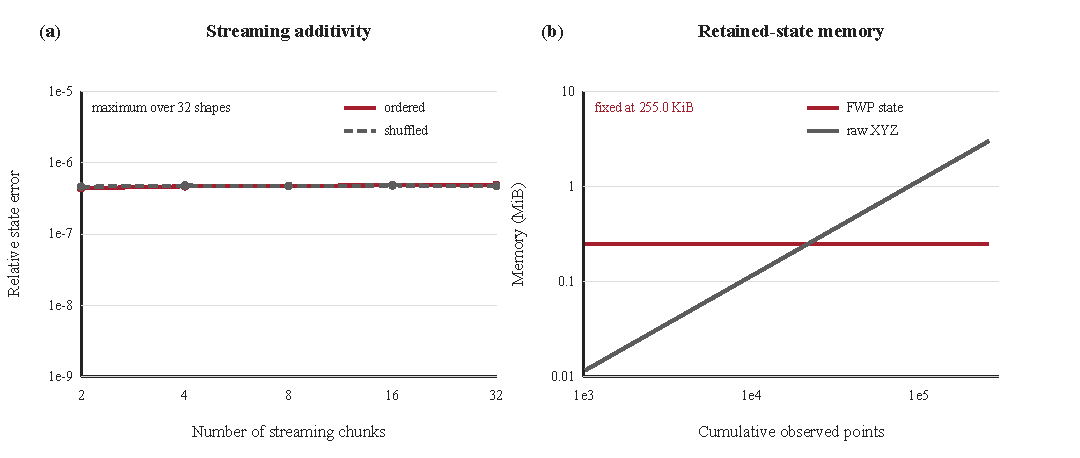
\includegraphics[width=0.92\linewidth]{fig01_additivity_fixed_state.pdf}
\caption{Additive streaming and fixed retained memory. Ordered and shuffled chunk writes reproduce the single-batch FWP state up to floating-point accumulation error. The three $128\times170$ float32 states occupy 255 KiB regardless of stream length, whereas stored XYZ coordinates grow linearly with the number of observations.}
\label{fig:additivity_fixed_state}

\end{figure}

\begin{figure}[t]\centering
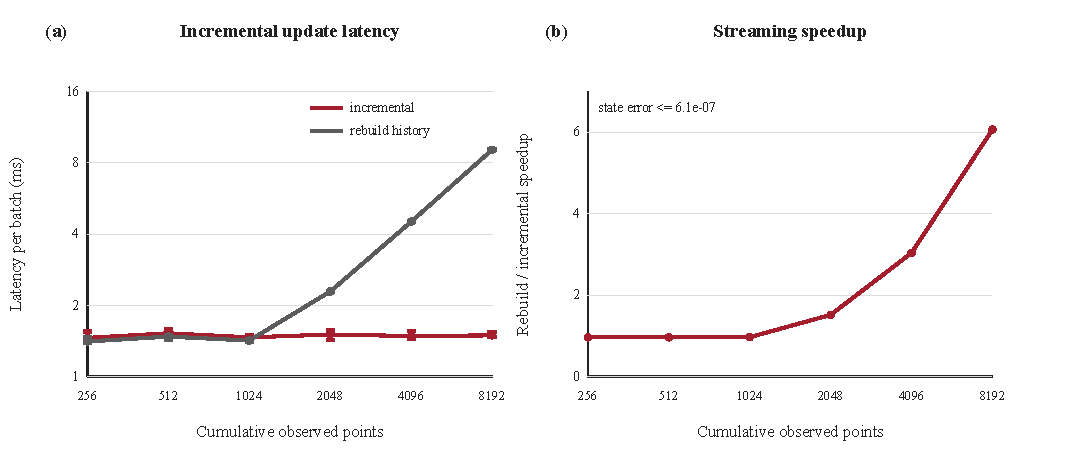
\includegraphics[width=0.92\linewidth]{fig04_streaming_efficiency.pdf}
\caption{FWP state-construction cost for device-resident point streams. (a) An incremental update processes one new 256-point frame, whereas reconstruction processes every accumulated point. Values are median wall-clock latency over seven interleaved trials of 30 repetitions for four streams; whiskers show the observed range. (b) The speedup grows with history length, while incremental and reconstructed states remain numerically equivalent.}
\label{fig:streaming-efficiency}

\end{figure}
On an RTX 3070 Ti Laptop GPU, four streams receive 256 new points per frame. Incremental latency stays near 1.46--1.53 ms, whereas reconstruction grows with history. Updating becomes $1.52\times$, $3.04\times$, and $6.06\times$ faster at 2,048, 4,096, and 8,192 accumulated points. Below roughly 512 accumulated points the two paths cost the same and rebuilding is marginally faster, so the advantage is asymptotic rather than universal.

\subsection{State algebra in practice}
\begin{figure}[t]\centering
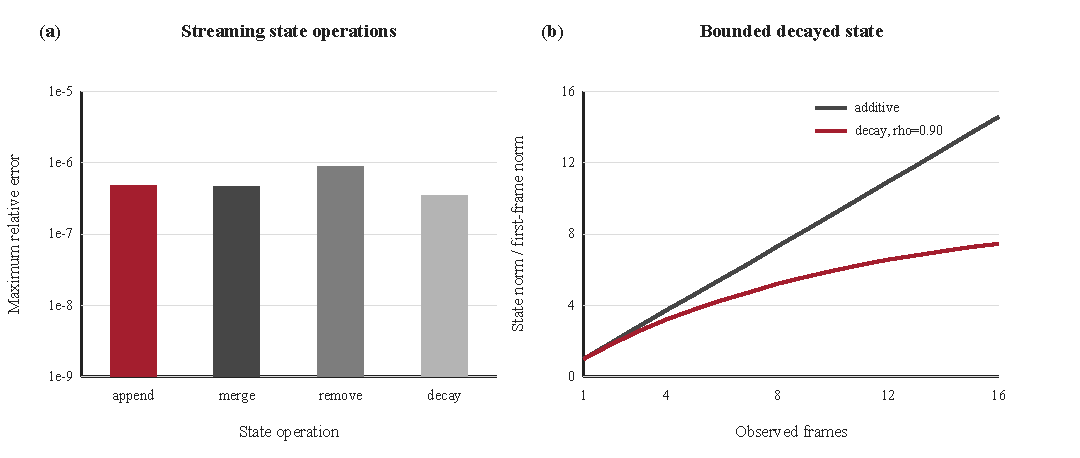
\includegraphics[width=0.92\linewidth]{fig02_state_operations.pdf}
\caption{Streaming state operations. (a) Maximum relative errors for append/merge, frame removal, and exponential decay, measured against independently reconstructed FWP states on 32 ShapeNetPart objects. (b) Ordinary addition increases the state magnitude with the number of frames, while exponential decay limits the influence of older frames without changing state size.}
\label{fig:streaming-state-operations}

\end{figure}
Append, independently encoded merge, stored-frame removal, and exponential decay were compared with direct reconstruction on 32 ShapeNetPart objects. Their mean relative errors were $2.11\times10^{-7}$, $2.13\times10^{-7}$, $3.03\times10^{-7}$, and $1.77\times10^{-7}$, respectively, and all maxima were below $9.8\times10^{-7}$. The remaining discrepancy is consistent with float32 accumulation order. After 16 frames, ordinary addition produced state norm 14.51; decay with $\rho=.9$ limited the norm to 7.42. This experiment validates the state equations and does not claim temporal-task accuracy.

\subsection{Controlled screens for the final heads}
\label{sec:screens}
\begin{figure}[t]\centering
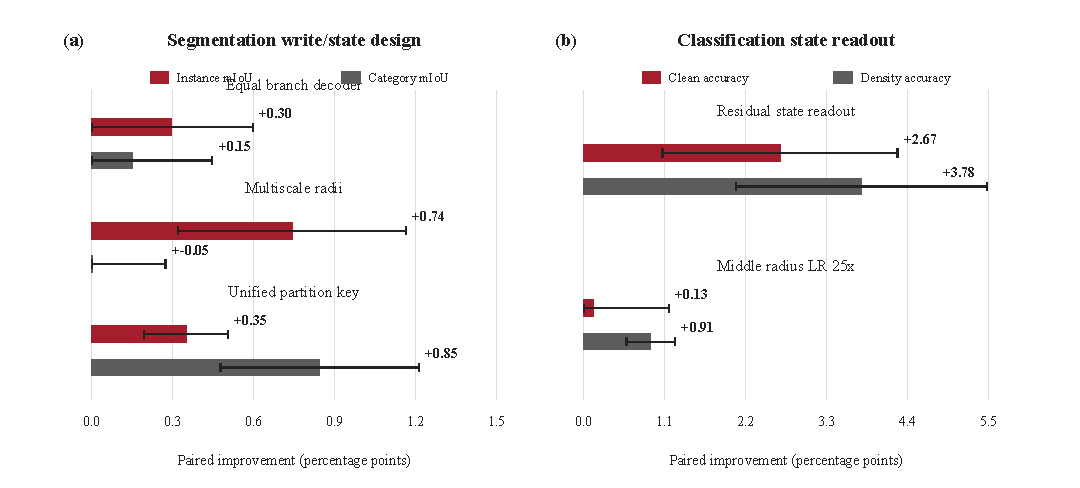
\includegraphics[width=0.92\linewidth]{fig03_controlled_ablation.pdf}
\caption{Three-seed, five-epoch architecture screens. Bars show paired mean changes and whiskers show population standard deviations. Segmentation tests equal branch decoders, distinct radius initialization, and a common normalized spatial address. Classification tests residual versus concatenated branch summaries and the middle-radius learning rate.}
\label{fig:architecture-ablation-main}
\end{figure}
The screens isolate one architectural decision at a time. All of them use the same data split and optimization protocol within a comparison, five epochs, seeds 0, 1, and 2, and a subset of 2,048 training and 512 test shapes. These short runs select structural choices; the main tables report final 20-epoch results on the complete splits. \Cref{tab:screens} reports paired changes of the retained design relative to the named alternative.

\begin{table}[t]
\centering
\caption{Controlled five-epoch screens. Positive changes favor the retained design.}
\label{tab:screens}
\small
\begin{tabular}{p{0.27\linewidth}p{0.25\linewidth}p{0.36\linewidth}}
\toprule
Retained choice & Paired alternative & Paired change\\
\midrule
Seg.: equal decoders & unequal middle decoder & $+0.30\pm0.30$ instance; $+0.15\pm0.29$ category\\
Seg.: distinct radius starts & equal radius starts & $+0.74\pm0.42$ instance; $-0.05\pm0.33$ category\\
Seg.: common normalized key & mixed key definitions & $+0.35\pm0.16$ instance; $+0.85\pm0.37$ category\\
Cls.: middle residual & direct concatenation & $+2.67\pm1.60$ clean; $+3.78\pm1.71$ shifted\\
Cls.: $25\times$ middle-radius LR & base radius LR & $+0.13\pm1.03$ clean; $+0.91\pm0.33$ shifted\\
\bottomrule
\end{tabular}
\end{table}

Equal $170\rightarrow160\rightarrow160$ segmentation decoders improve instance mIoU by $0.30\pm0.30$ points and remove 24,480 parameters. Distinct radius initialization improves instance mIoU by $0.74\pm0.42$. Applying the same normalized address equation to all three branches improves instance and category mIoU by $0.35\pm0.16$ and $0.85\pm0.37$ over a mixed-key variant. For state-only classification, the middle-reference residual improves clean and density-shift accuracy by $2.67\pm1.60$ and $3.78\pm1.71$ over direct concatenation. Increasing only the middle-radius learning rate gives a variable clean-accuracy change but a consistent $0.91\pm0.33$ shifted-accuracy gain; it is retained for that consistent gain rather than for its clean-accuracy effect. These results motivate the released heads while keeping the state-writing rule symmetric across branches.

\section{Discussion and Limitations}
The intended setting is a growing or distributed point stream. A sensor can encode a frame, merge its state, and release the frame. Several cameras, LiDARs, robots, or edge processors can encode disjoint spatial regions or time windows locally and send fixed states to a server. Addition then produces the same representation as centralized encoding, so aggregation can be asynchronous and hierarchical. Raw point sets need not leave the sensing devices. A segmentation service can retain only coordinates it plans to query, while a classifier updates its evidence without replaying earlier points. None of these operations compares a new point with all previously decoded points.

\subsection{Worked distributed inference}
Consider several LiDAR nodes observing different parts of a scene. The trained encoder is copied to every node, and all nodes express coordinates in a common frame with the same normalization. Node $d$ encodes its local chunk into $\{\Sstate_f^{(d)},\Sstate_m^{(d)},\Sstate_b^{(d)}\}$ and can then delete the local features. A relay may add any subset of these triples; the server adds the relay outputs and obtains Equation~\eqref{eq:distributed-main}. The order of arrival and the shape of the communication tree do not affect the real-arithmetic result. Each transmitted triple has the same 255 KiB size whether the local chunk contains hundreds of points or represents a long accumulated stream.

For classification, the server passes the merged triple directly to the state-row readout. A new device or frame changes the class evidence by adding one more triple, without decoding and pooling the earlier clouds again. For segmentation, the server supplies a coordinate $\bm q$ to the three matrix reads. Queries may be the coordinates of selected observed points, a region requested by an operator, or positions on a regular grid. Only these coordinates need to be available at read time. Because Equation~\eqref{eq:effective-read-main} depends smoothly on $\bm q$, nearby queries receive smoothly changing state evidence, including at coordinates that were not explicitly observed. The current experiments evaluate labels only at observed ShapeNetPart points, so accuracy at new coordinates remains an open empirical question.

\subsection{What the fixed state retains and discards}
\label{sec:bottleneck}
The fixed states are summaries rather than compressed point archives. They are sufficient to evaluate the learned heads, but they are not designed to reconstruct every original observation. Two point sets can produce similar moment tables, especially when many spatial addresses overlap. The learned centers, radii, content networks, and second-order terms determine which distinctions survive this compression. This explains both the bounded-memory benefit and the remaining accuracy gap to a neighborhood method that retains or rebuilds detailed point relations.

More precisely, once a point has been written the state is the only thing any later stage can see, so no decoder can restore a distinction that the write has already discarded. The state, and not the readout, is the binding compression bottleneck of the architecture. The screens support this directly. Changing the segmentation decoders moves instance mIoU by $0.30\pm0.30$ points, and changing their width or sharing pattern produces similar sub-point changes, whereas changing the state configuration in \Cref{sec:parallel} moves it by more than one point. This is why the design spends its structure on how points are written -- the normalized address, the second-order value, and the use of several parallel states -- rather than on how the state is decoded, and it is the reason a wider main state is a poor substitute for the parallel structure.

PointNet++ forms neighborhoods around observed points and PointNet preserves channelwise extremes, whereas PointProgrammerNet retains finite moment tables. The state also exceeds bare-XYZ storage for short clouds; its benefit appears when bounded communication, merging, or long streams justify the fixed cost. Distributed equivalence requires identical preprocessing and a shared coordinate frame, and segmentation still reads the state once per requested coordinate. Evaluation is limited to XYZ input, one dataset per task, one timing GPU, and local controlled baselines. Unseen-query accuracy, temporal calibration, additional attributes, and delta adaptation remain future work.

\section{Conclusion}
PointProgrammerNet summarizes a point cloud with fixed additive matrices. Continuous keys and second-order values support unordered writes, exact distributed merging, removal, decay, and updates whose cost does not depend on history length. Several parallel states encode more usable structure than a single state of the same parameter budget, and the state itself is the binding compression bottleneck, not the readout. Coordinate-conditioned segmentation and state-only classification operate without pooling over decoded points. The model provides a compact and testable design for centralized or distributed point-cloud inference from a bounded streaming state, at an accuracy cost relative to hierarchical baselines that the experiments quantify.

\section*{Statements and Declarations}
\noindent\textbf{Competing interests.} The author declares no competing financial
or non-financial interests related to this work.

\noindent\textbf{Funding.} No funding was received for conducting this study.

\noindent\textbf{Author contributions.} Dian Yu: conceptualization, methodology,
software, validation, formal analysis, investigation, data curation,
visualization, writing -- original draft, writing -- review and editing.

\noindent\textbf{Data availability.} ShapeNetPart and ModelNet40 are public
datasets available from the original sources cited in this article. The released
minimal code contains the 341,909-parameter segmenter and the
529,426-parameter classifier, dataset loaders, training loops, state-operation
checks, and exact three-seed reference values; \texttt{CODE\_REPRODUCTION.md}
specifies the environment, dataset layout, commands, and streaming API.
Additivity tests should be run in evaluation mode, because BatchNorm then uses
the fixed running statistics assumed by \Cref{prop:order}.

\bibliographystyle{unsrt}
\bibliography{references}
\end{document}
